\documentclass[tikz]{standalone}
\usetikzlibrary{calc}

\begin{document}

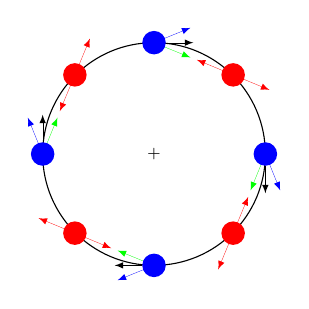
\begin{tikzpicture}[>=latex,
cnode/.style={circle,inner sep=3pt,outer sep=0},
myline/.style={ultra thin,->}
]
\def\myarrowlen{5mm}
\pgfmathsetmacro{\myradius}{sqrt(2)}

\node[draw,circle,minimum size=2*\myradius cm] (bigc) at (0,0) {\tiny +};

\foreach \x in {1,...,8}{
\ifodd\x\relax
    \node[cnode,fill=red] (n-\x) at (bigc.45*\x) {};
    \draw[red,myline] (n-\x)  -- ($(n-\x)!-\myarrowlen!(bigc.45*\x+45)$);
    \draw[red,myline] (n-\x)  -- ($(n-\x)! \myarrowlen!(bigc.45*\x+45)$);
\else
    \node[cnode,fill=blue] (n-\x) at (45*\x:\myradius) {};
    \draw[blue , myline] (n-\x) -- ($(n-\x)!-\myarrowlen!(bigc.45*\x+45)$);
    \draw[green, myline] (n-\x) -- ($(n-\x)! \myarrowlen!(bigc.45*\x-45)$);
    \draw[     , myline] (n-\x) -- ++({45*(\x-2)}:\myarrowlen);
\fi
}
\end{tikzpicture}
\end{document}
